\documentclass[tikz,border=5pt]{standalone}
\usepackage[T1]{fontenc}
\usepackage{lmodern,amsmath,amssymb}
\usetikzlibrary{arrows.meta,calc,positioning,fit,backgrounds,shapes.geometric,matrix,decorations.pathreplacing,patterns}
\definecolor{ink}{gray}{0.08}
\definecolor{wash}{gray}{0.965}
\definecolor{soft}{gray}{0.45}
\tikzset{box/.style={draw=ink,line width=.65pt,fill=white,align=center,inner sep=4pt,outer sep=0pt,font=\small},flow/.style={draw=ink,line width=.65pt,-{Latex[length=1.8mm,width=1.3mm]},rounded corners=2pt},annotation/.style={font=\scriptsize,text=soft,align=center},groupbox/.style={draw=soft,dashed,line width=.45pt,fill=wash}}
\begin{document}
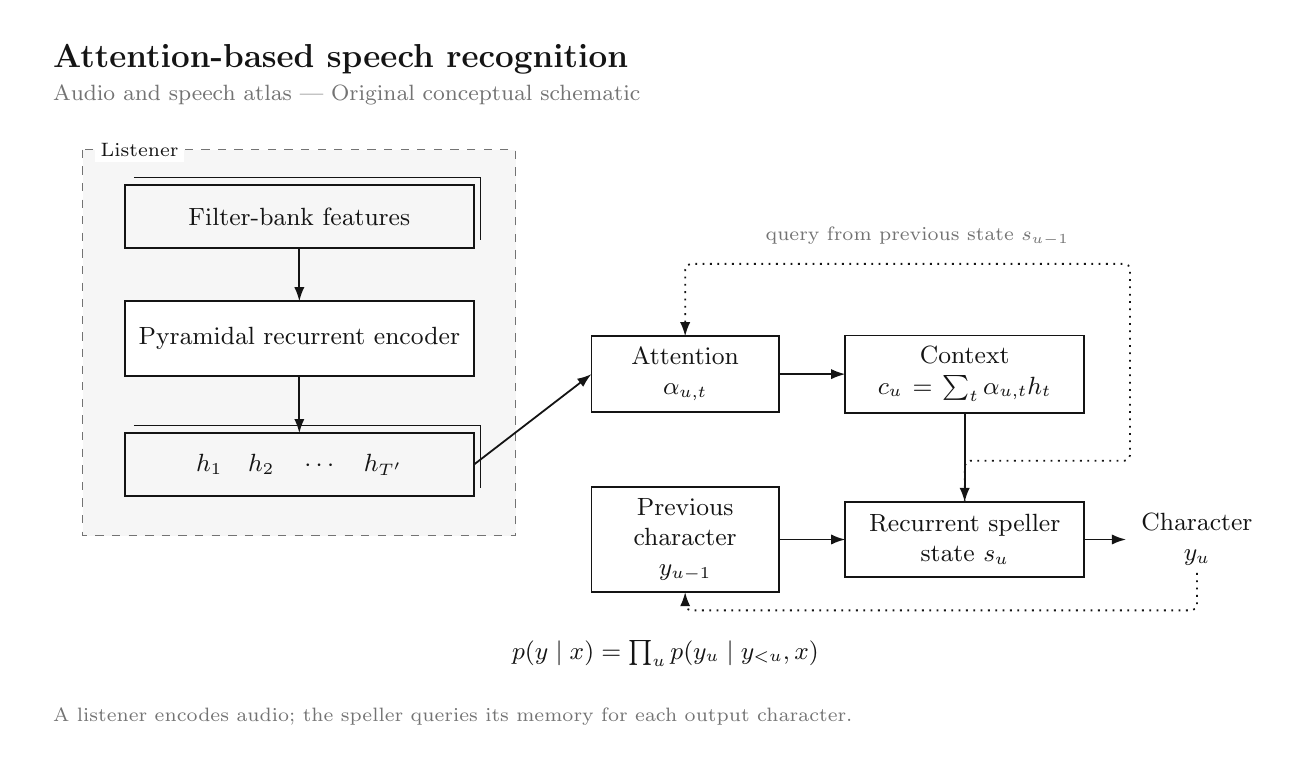
\begin{tikzpicture}[x=1cm,y=-1cm,font=\rmfamily,text=ink]

\path[use as bounding box] (0,0) rectangle (16,9);
\node[anchor=west,font=\large\bfseries] at (.2,.4) {Attention-based speech recognition};
\node[anchor=west,font=\footnotesize,text=soft] at (.2,.85) {Audio and speech atlas | Original conceptual schematic};
\begin{pgfonlayer}{background}
\draw[groupbox] (0.7,1.55) rectangle (6.2,6.45);
\node[anchor=west,font=\scriptsize,fill=white,inner sep=2pt] at (0.85,1.55) {Listener};
\end{pgfonlayer}
\node[box,fill=wash,minimum width=4.4cm,minimum height=0.8cm,text width=4.15cm] (features) at (3.45,2.4) {Filter-bank features};
\draw[ink,line width=.4pt] (1.35,1.9) -- (5.75,1.9) -- (5.75,2.6999999999999997);
\node[box,minimum width=4.4cm,minimum height=0.95cm,text width=4.15cm] (listener) at (3.45,3.95) {Pyramidal recurrent encoder};
\node[box,fill=wash,minimum width=4.4cm,minimum height=0.8cm,text width=4.15cm] (memory) at (3.45,5.55) {$h_1\quad h_2\quad\cdots\quad h_{T'}$};
\draw[ink,line width=.4pt] (1.35,5.05) -- (5.75,5.05) -- (5.75,5.8500000000000005);
\node[box,minimum width=2.35cm,minimum height=0.95cm,text width=2.1cm] (attn) at (8.35,4.4) {Attention\\$\alpha_{u,t}$};
\node[box,minimum width=3.0cm,minimum height=0.95cm,text width=2.75cm] (context) at (11.9,4.4) {Context\\$c_u=\sum_t\alpha_{u,t}h_t$};
\node[box,minimum width=3.0cm,minimum height=0.95cm,text width=2.75cm] (decoder) at (11.9,6.5) {Recurrent speller\\state $s_u$};
\node[box,minimum width=2.35cm,minimum height=0.95cm,text width=2.1cm] (prev) at (8.35,6.5) {Previous character\\$y_{u-1}$};
\node[align=center,inner sep=0pt,outer sep=0pt,font=\small,minimum width=1.8cm,minimum height=0.85cm,text width=1.55cm] (char) at (14.85,6.5) {Character\\$y_u$};
\begin{pgfonlayer}{background}
\draw[flow] (features.south) -- (listener.north);
\draw[flow] (listener.south) -- (memory.north);
\draw[flow] (memory.east) -- (attn.west);
\draw[flow] (attn.east) -- (context.west);
\draw[flow] (context.south) -- (decoder.north);
\draw[flow] (prev.east) -- (decoder.west);
\draw[flow] (decoder.east) -- (char.west);
\draw[flow,dotted] (decoder.north) -- (11.9,5.5) -- (14.0,5.5) -- (14.0,3.0) -- (8.35,3.0) -- (attn.north);
\draw[flow,dotted] (char.south) -- (14.85,7.4) -- (8.35,7.4) -- (prev.south);
\end{pgfonlayer}
\node[align=center,anchor=center,font=\scriptsize,text=soft,text width=6cm] at (11.3,2.65) {query from previous state \mbox{$s_{u-1}$}};
\node[align=center,anchor=center,font=\small,text=ink,text width=13cm] at (8.1,7.95) {\mbox{$p(y\mid x)=\prod_u p(y_u\mid y_{<u},x)$}};
\node[anchor=west,align=left,font=\scriptsize,text=soft,text width=15.6cm] at (.2,8.75) {A listener encodes audio; the speller queries its memory for each output character.};
\end{tikzpicture}
\end{document}
